\begin{figure*}[htb]
\centering
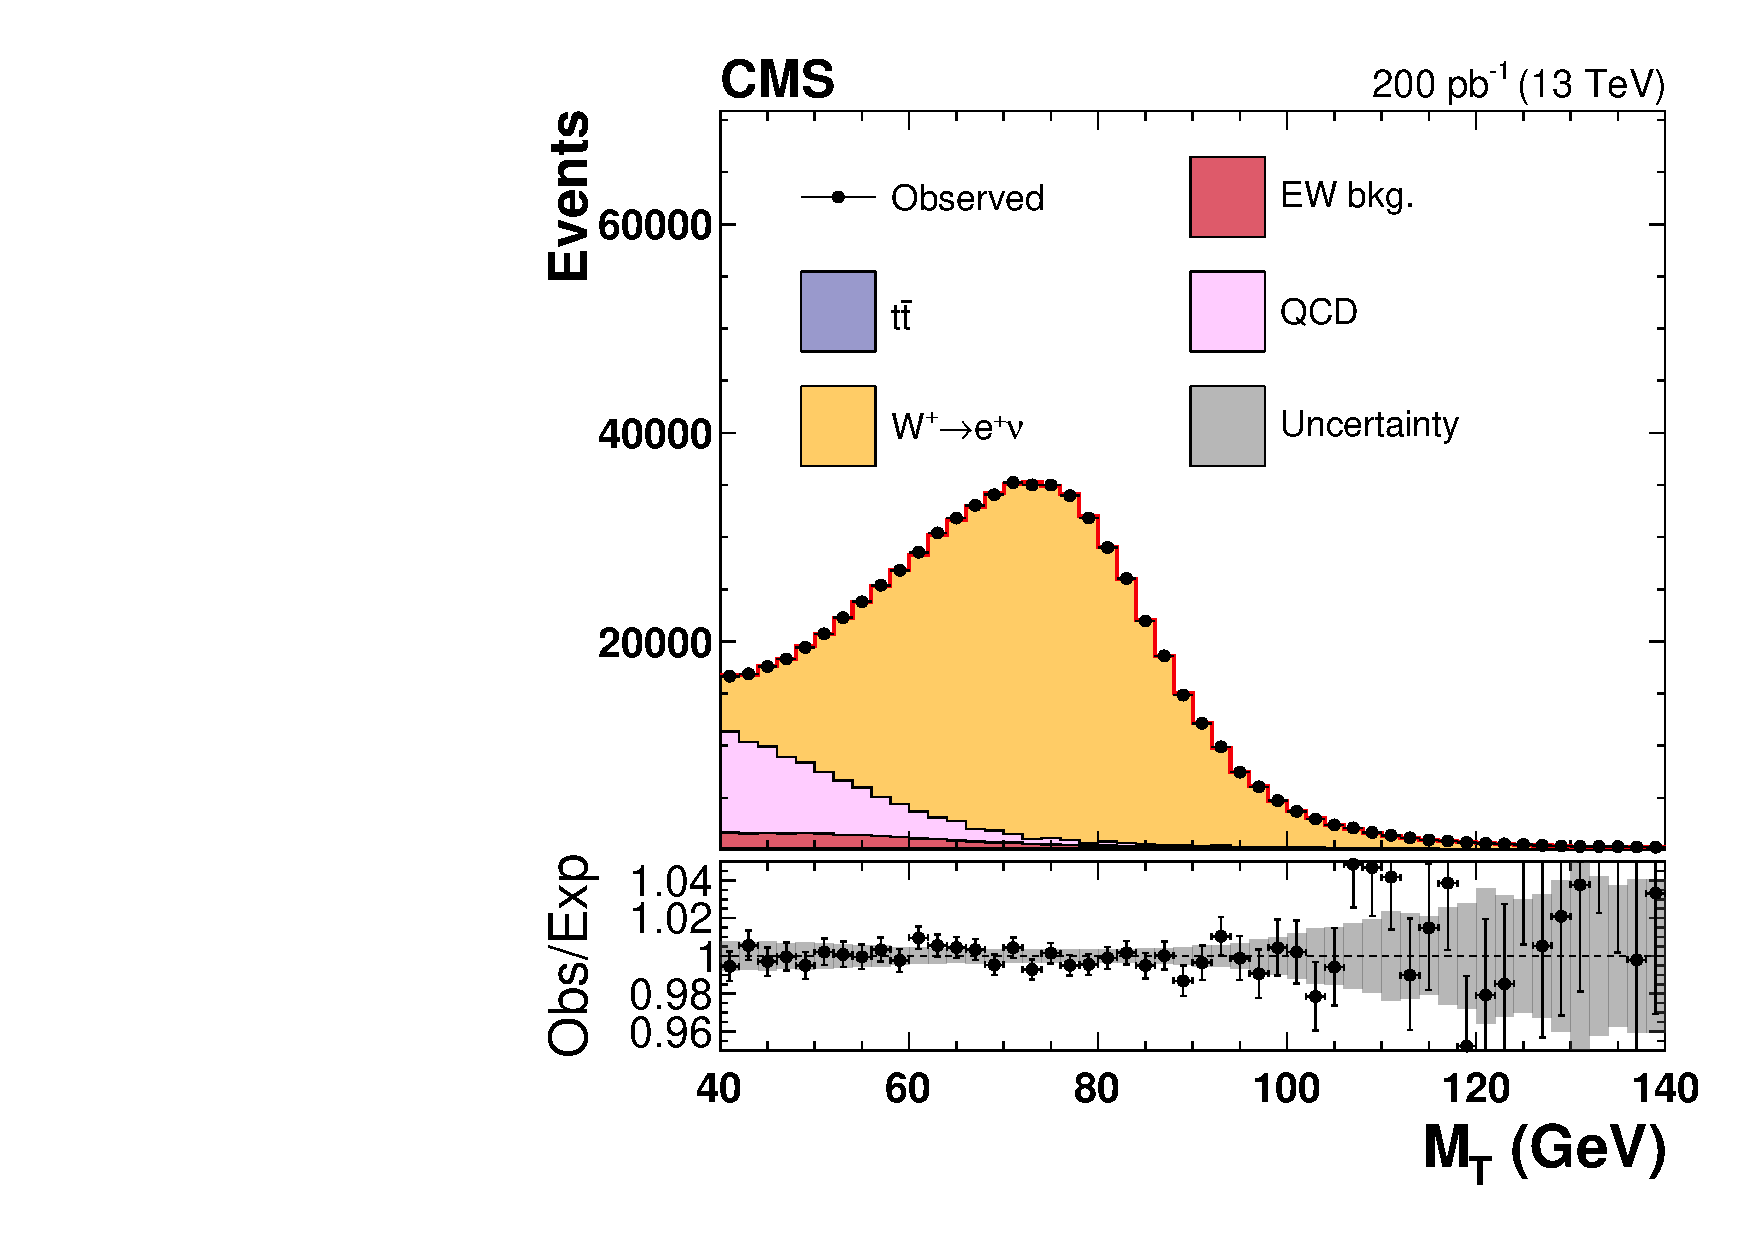
\includegraphics[width=0.49\textwidth]{plots/W/wpefit13.pdf}
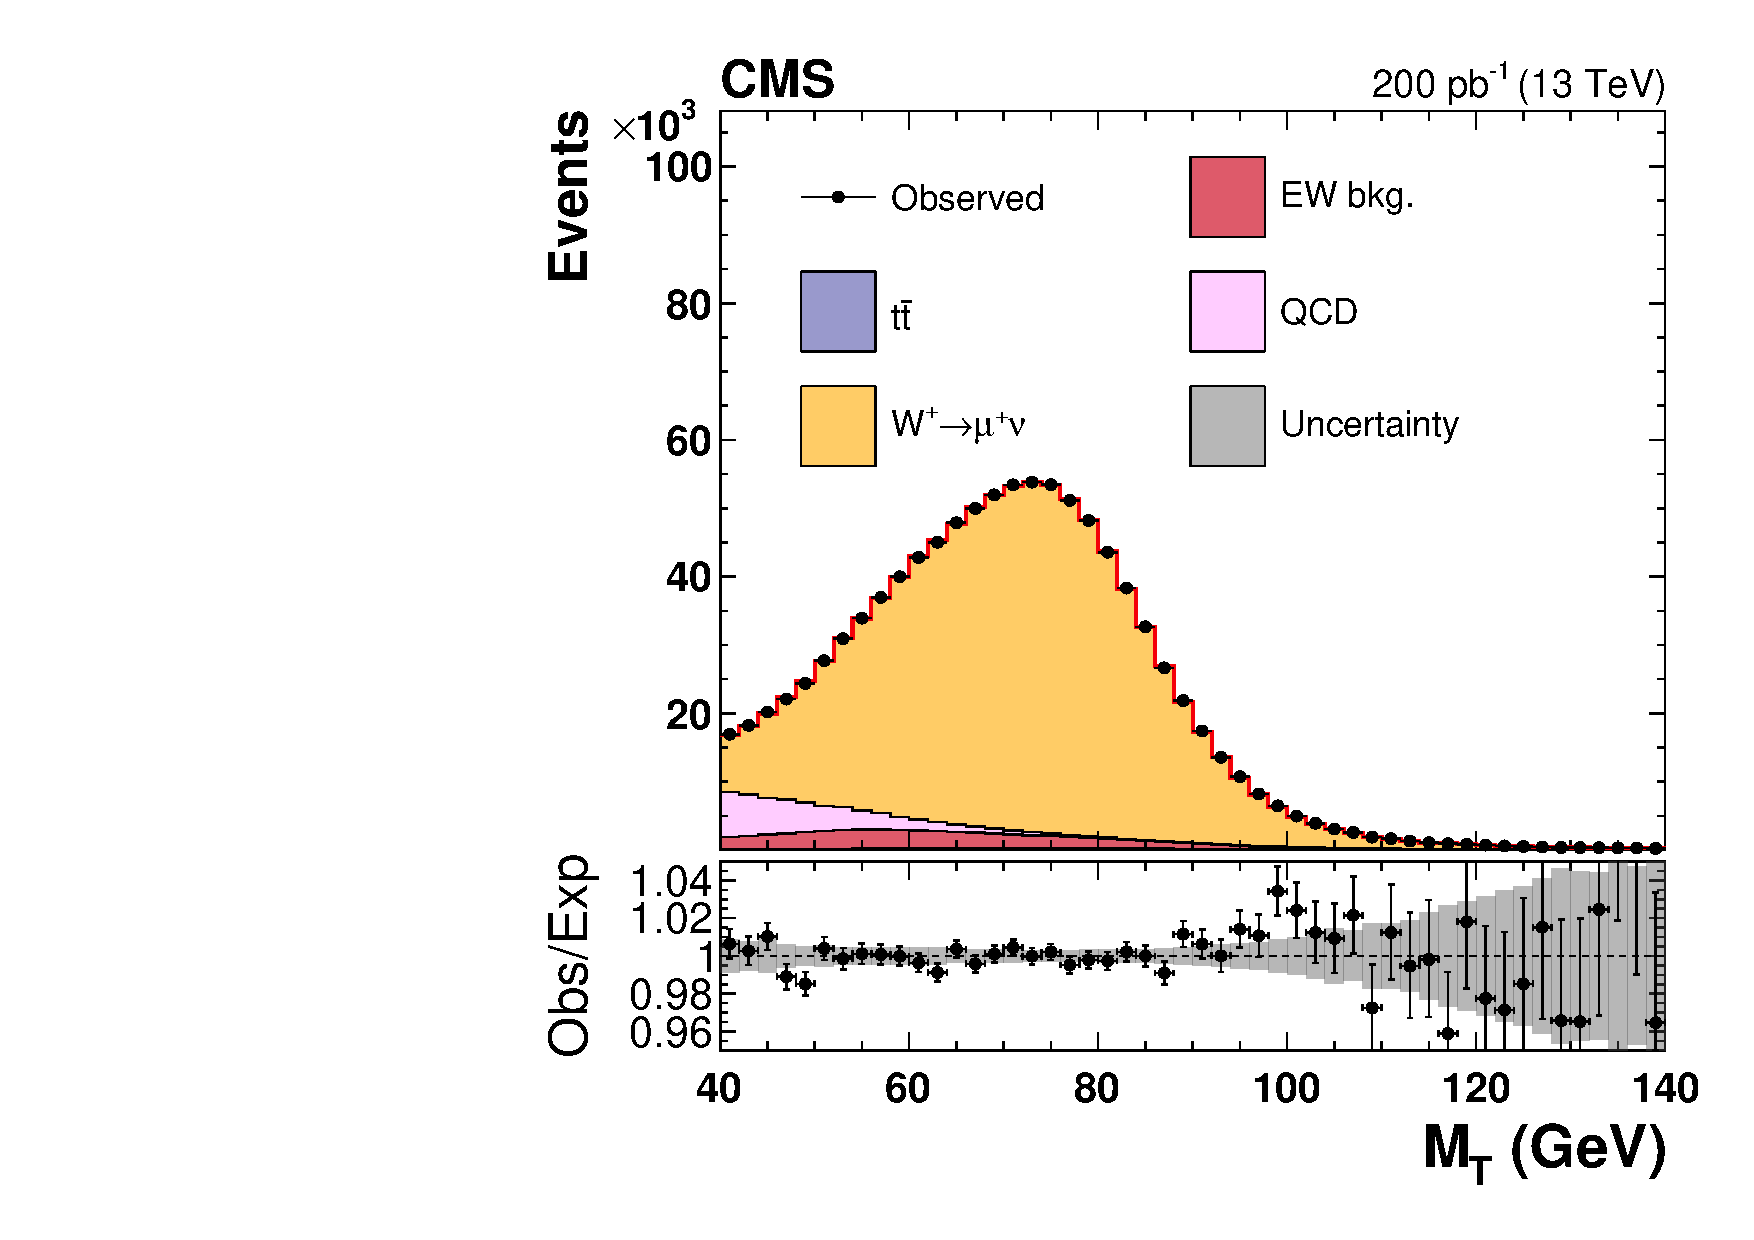
\includegraphics[width=0.49\textwidth]{plots/W/wpmfit13.pdf}
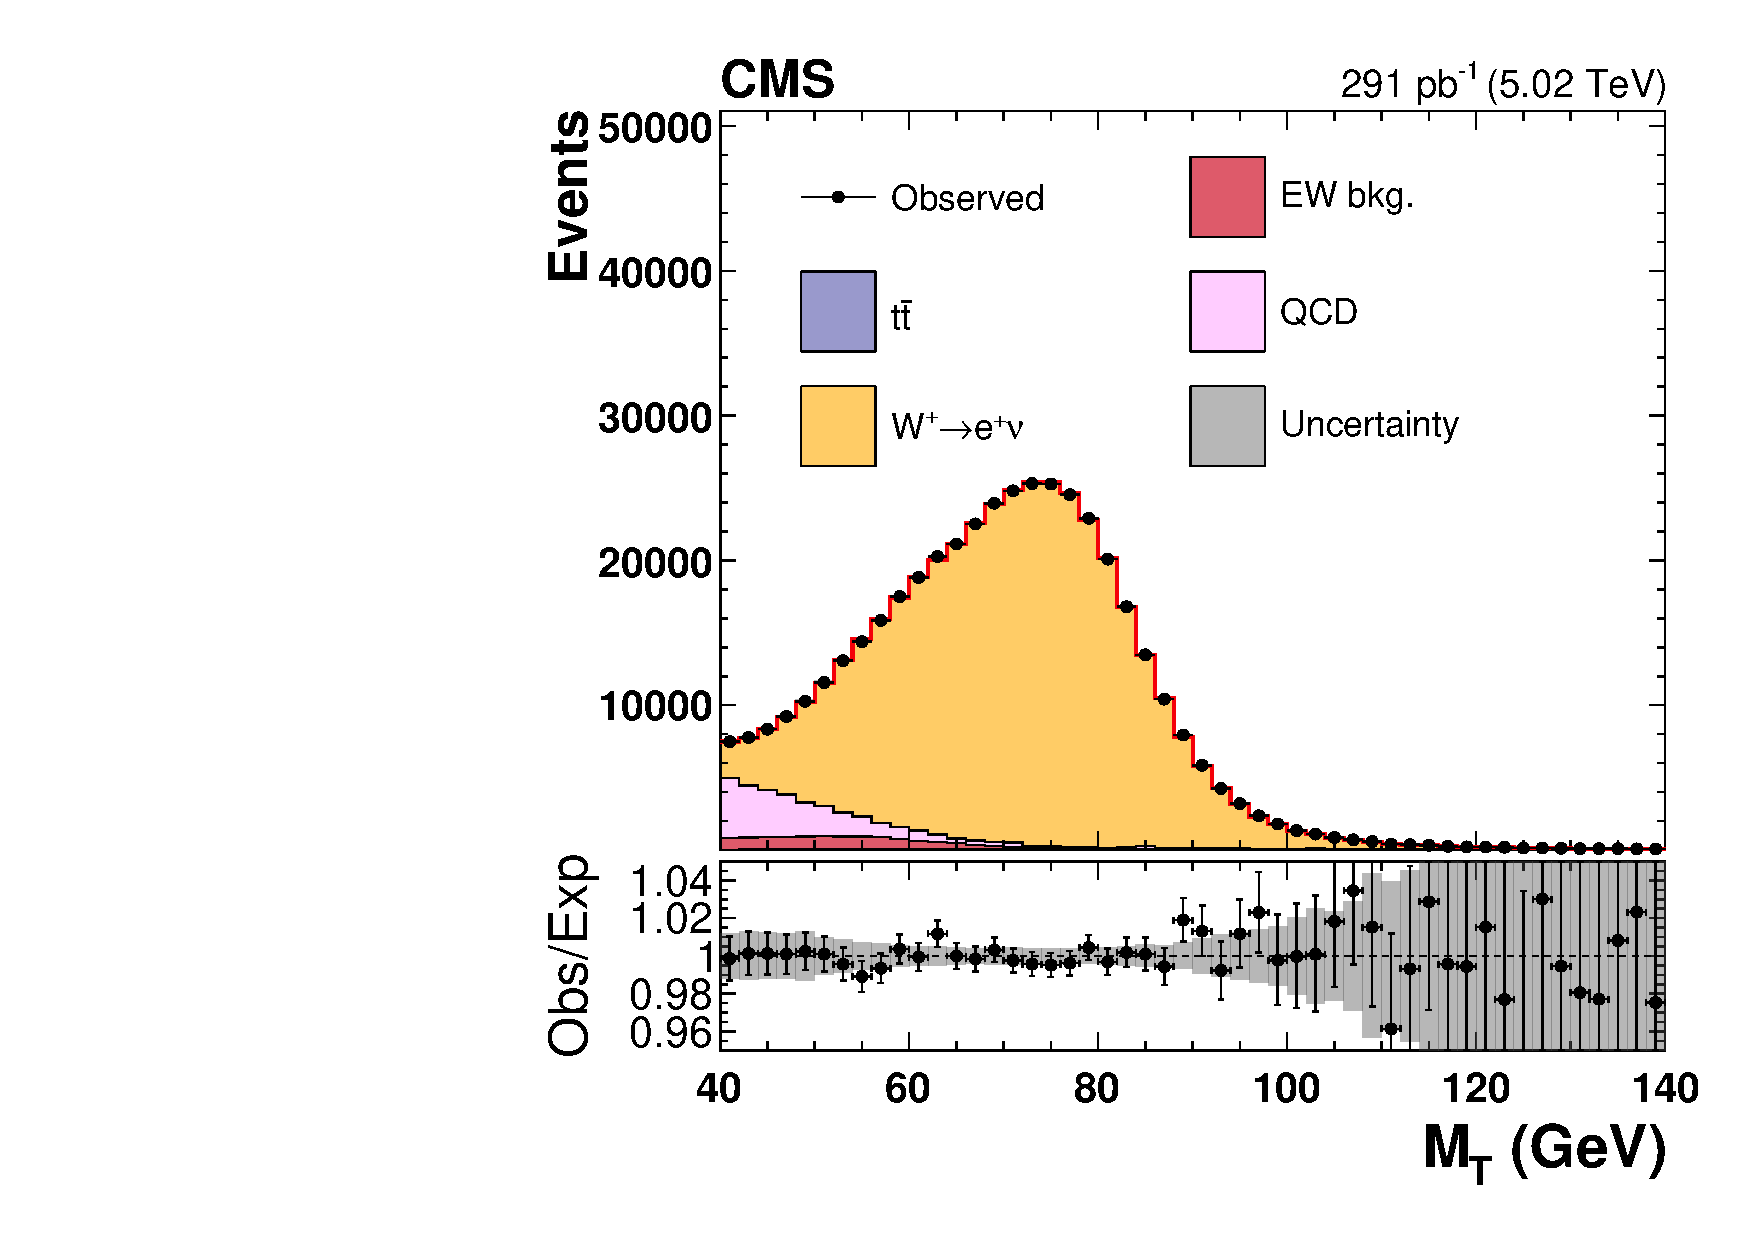
\includegraphics[width=0.49\textwidth]{plots/W/wpefit5.pdf}
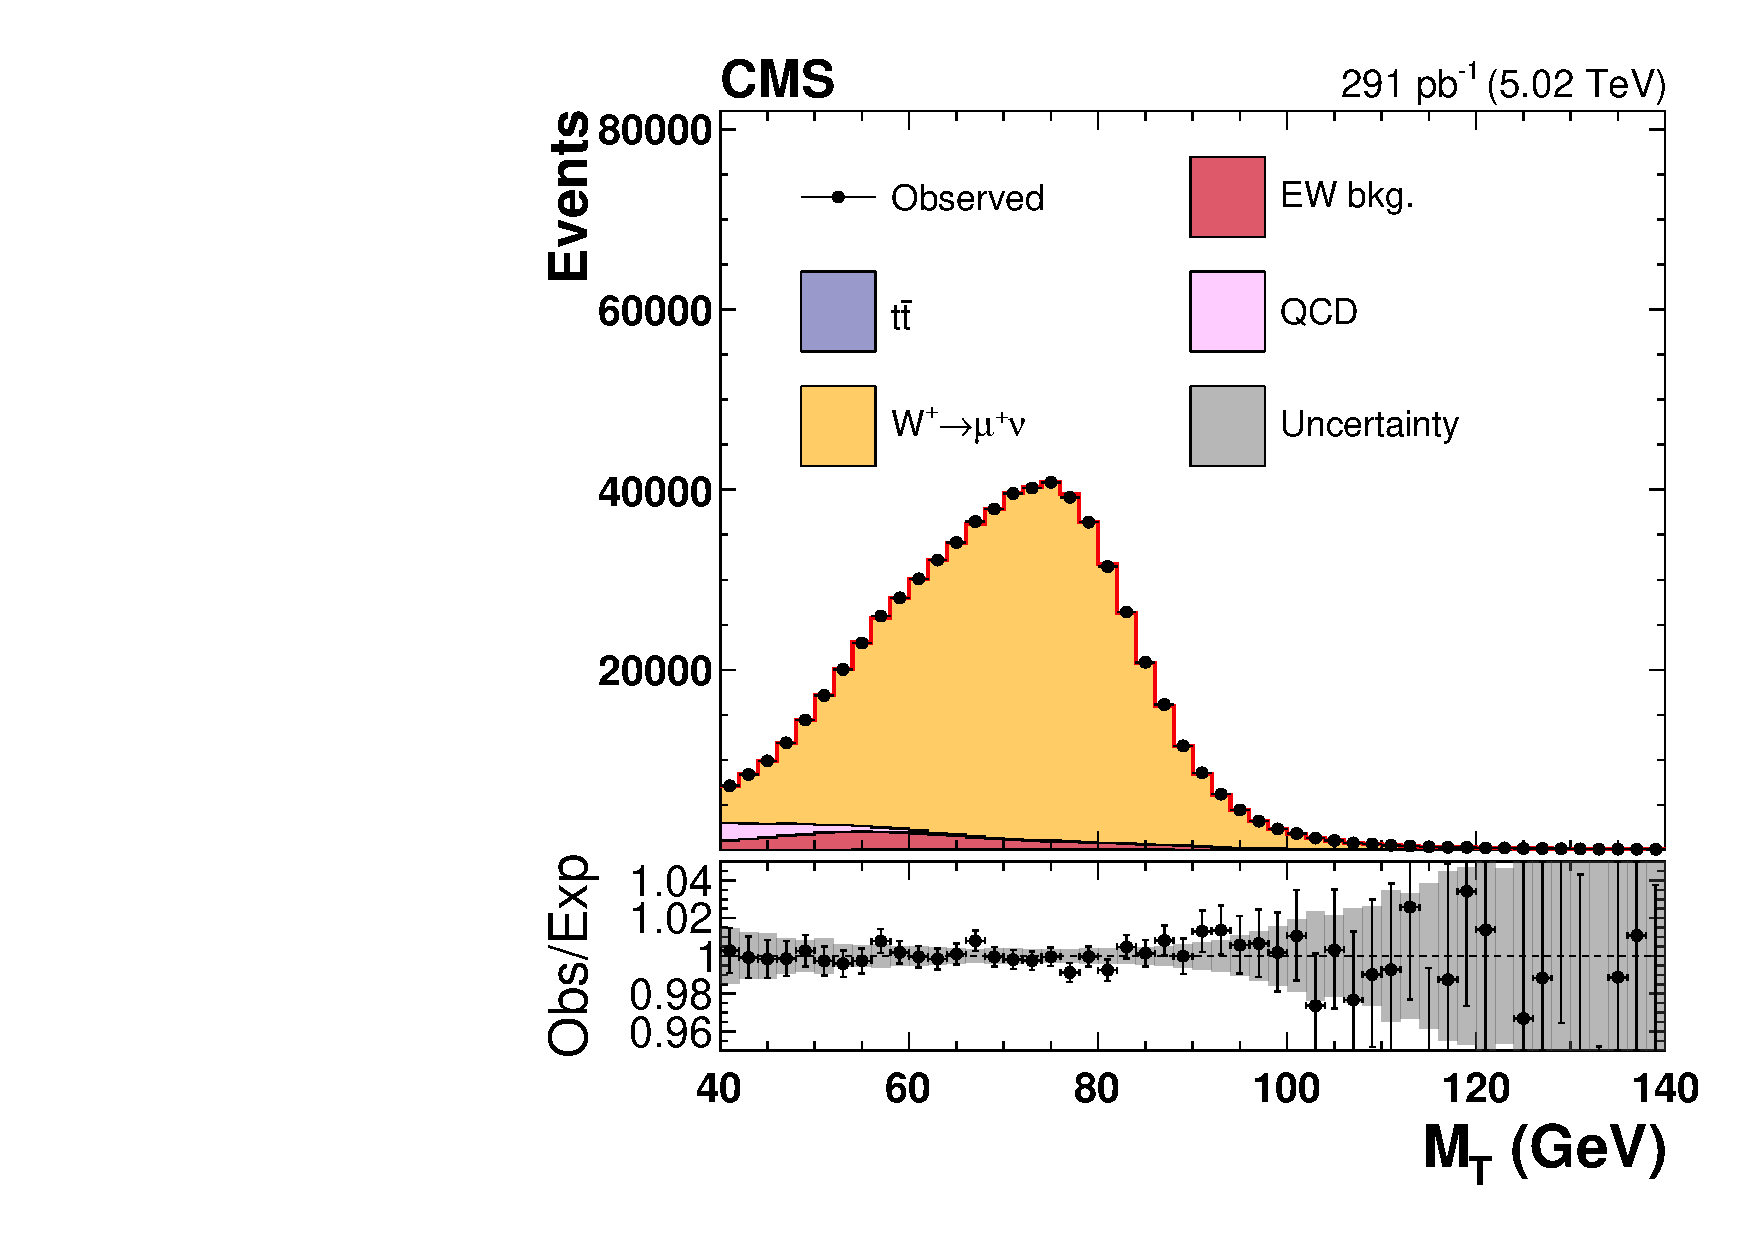
\includegraphics[width=0.49\textwidth]{plots/W/wpmfit5.pdf}
\caption{Distributions of \mt in the $\W^{+}$ signal selection for electron (left) and muon (right) final states for the $pp$ collisions at $\sqrt{s}=13\TeV$ (upper) and $\sqrt{s}=5.02\TeV$ (lower). The histograms for EW backgrounds include the contributions from Drell--Yan, $W \to \tau\nu$, and diboson processes. The predicted yields are shown with their best-fit normalizations from the fit. The bottom panel in each figure shows the ratio of the number of events observed in data to that of the total signal and background predictions.}
\label{fig:signal_wp}
\end{figure*}